\documentclass{article}

%% Page Margins %%
\usepackage{geometry}
\geometry{
    top = 0.75in,
    bottom = 0.75in,
    right = 0.75in,
    left = 0.75in,
}

\usepackage{amsmath}
\usepackage{graphicx}
\usepackage{parskip}

\title{Project Report: Milestone 1}

\author{Janssen Myer Rambaud (1008107004), Felix Zhang (1007650212)}

\begin{document}
\maketitle

\section{Part I: Planning and Configuration}

\begin{enumerate}
\item Breakout Plan:

\item Translate your plan into the .data section of your breakout.asm program. Assemble your program in MARS and inspect memory to ensure it matches your plan. Include a screenshot (or multiple screenshots) of memory demonstrating that it has been laid out according to your plan.

\begin{figure}[ht!]
    \centering
    % \includegraphics[width=0.8\textwidth]{milestone1_memory.png}
    \caption{Screenshot of memory.}
    \label{f:part1_memory_writer}
\end{figure}

\newpage

\section{Part II: Milestone 1}

\item Draw the scene (Milestone 1)

\begin{figure}[ht!]
    \centering
    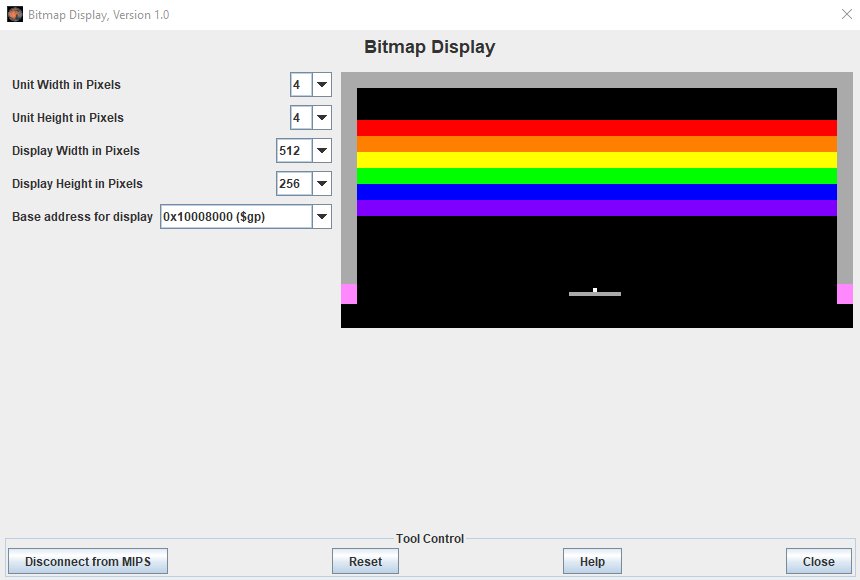
\includegraphics[width=0.8\textwidth]{milestone1_drawing.png}
    \caption{The static scene of Milestone 1 Drawing.}
    \label{f:milestone1_drawing}
\end{figure}

\end{enumerate}


\newpage

\section{Part III: Milestone 2}

\item \textbf{QUESTION: } How will the ball change directions when it collides?
\item Upload breakout.asm to MarkUs so that you have a snapshot of your progress so far.

\section{Part IV: Milestone 3}
\item Upload breakout.asm to MarkUs so that you have a snapshot of your progress so far.
\end{document}